\section{Robustness Checks}
\subsection{Robustness Checks (long) }
 We examine the sub sample of countries which experienced a high level of unemployment growth, high level of debt growth and a low level of GDP growth during the years after the great recession and the European debt crisis namely from 2007 to 2012. We also consider Southern European countries, countries located more at the periphery \footnote{as measured by distance form Brussels} and part of the Eurozone. The baseline results remain unchanged among these sample splits. When asked about the intentions behind entering the rescue program inferences of the baseline model do not change. The effect in the sample of countries with high levels of unemployment becomes smaller and is only significant at the five percent level. In the sample of southern European countries the disagreement over whether lender countries wanted to impose institutional change on borrower countries also decreases and is only significant at the five percent level. The estimates for the sample of periphery countries are larger than in the baseline sample. In the periphery sample participants from program countries are 19.1 percentage points less likely to agree with the statement that the lender countries wanted to help the borrowing countries and 14.2 percentage points more likely to agree that lender countries wanted to impose institutional change compared to 13.1 and 11.1 percentage points in the full sample.\\
When asked about the emotions of citizens in borrower and lender countries the estimates become slightly smaller in the southern European, periphery and high debt sample than for the full sample. The divergence in assessments about whether the rescue program made the citizens in the borrower countries feel inferior lacks statistical significance in the Southern European sample. Among both samples there is substantial disagreement between program and non-program countries that Greece will repay it's debt. 
\\
\begin{figure} [h!]
    \begin{center}
     \caption{ Intentions of the borrower countries}
    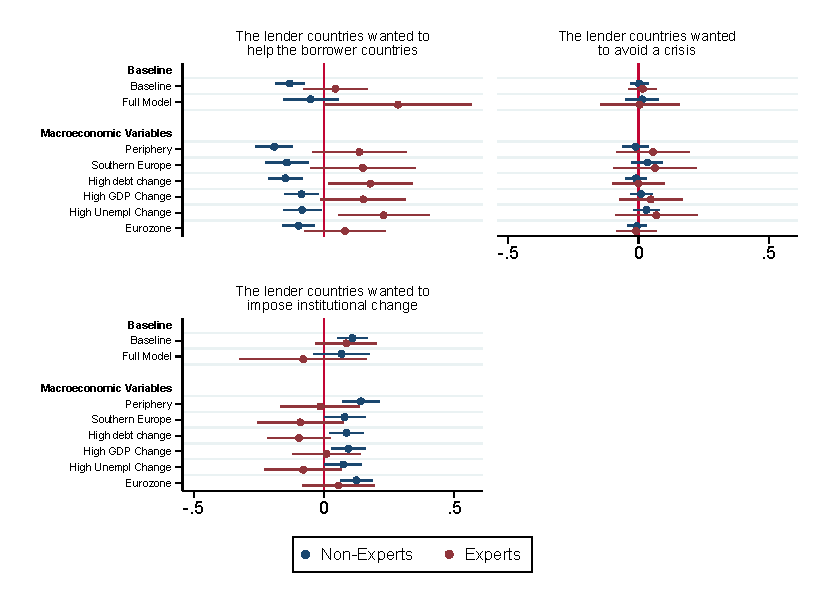
\includegraphics[scale=1.2]{Question2_samplesplits.pdf}
    \label{fig:my_label}
    \end{center}
    \tiny 
    \tablenotes{Participants were asked to assess the following statements:  Question 2.1: The lender countries wanted to help the borrowing countries Question 2.2: The lender countries wanted to help themselves avoid a crisis at home Question 2.3: The lender countries wanted to impose institutional change upon the borrower countries }
\end{figure}
\begin{figure}[h!]
    \begin{center}
     \caption{Sentiments of borrower countries (Macro Variables)}
    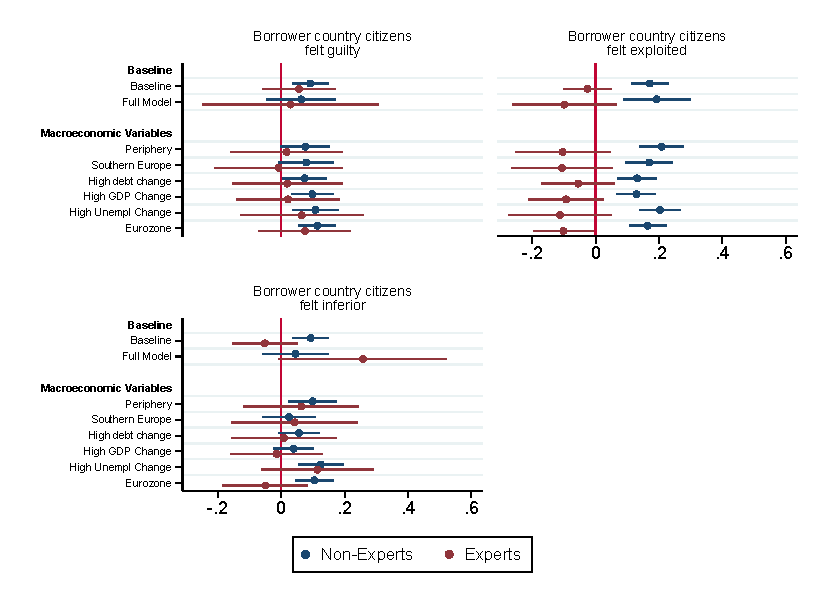
\includegraphics[scale=1.2]{Question51_samplesplits.pdf}
    \label{fig:my_label}
    \end{center}
    \tiny 
     \tablenotes{Question 5.1: The rescue experience made many citizens in the borrower countries feel guilty; Question 5.2: The rescue experience made many citizens in the borrower countries feel exploited; Question 5.3: The rescue experience made many citizens in the borrower countries feel inferior} 
\end{figure}
\begin{figure}[h!]
    \begin{center}
     \caption{Sentiments of lender countries(Macro Variables)}
    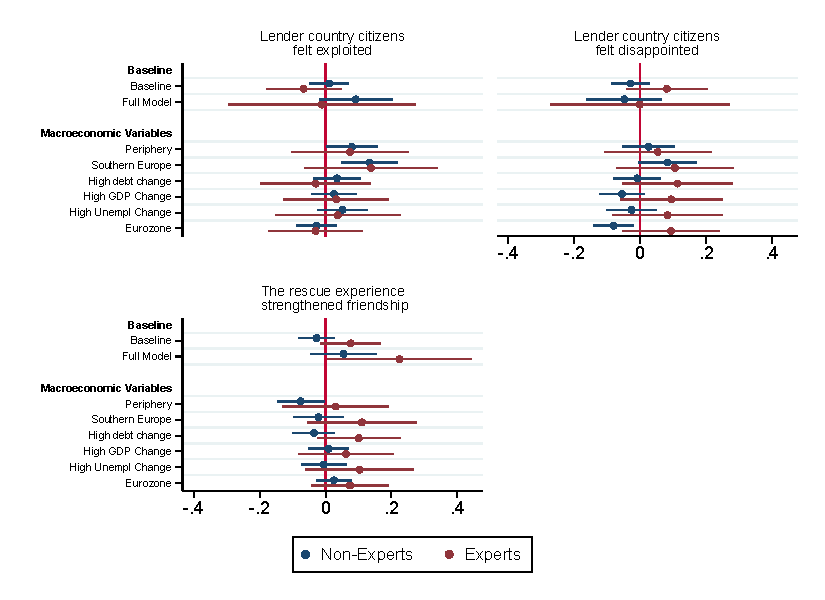
\includegraphics[scale=1.2]{Question52_samplesplits.pdf}
    \end{center}
    \tiny
     \tablenotes{Question 5.4: The rescue experience made many citizens in the lender countries feel exploited; Question 5.5 The rescue experience made many citizens in the lender countries feel disappointed Question 5.6: The rescue experience strengthened friendships between citizens Question 7: Greece will fully pay back it's debt}
\end{figure}
\begin{figure}[h!]
    \begin{center}
     \caption{Who initiated and benefited from the rescue program (Macro Variables)}
    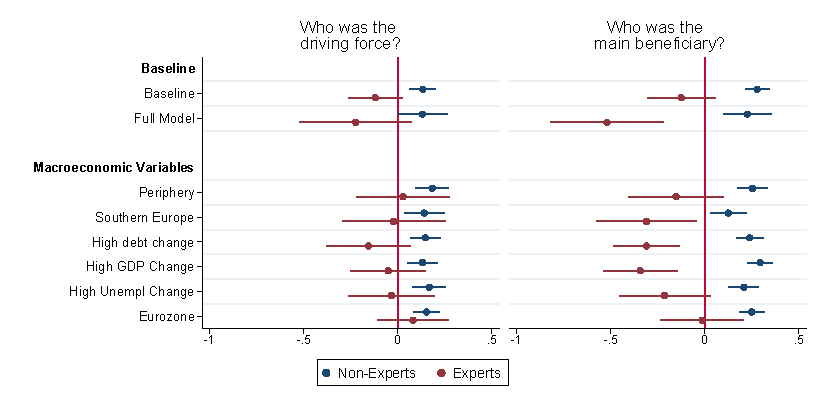
\includegraphics[scale=1.2]{macro_S_1301_S_1401.pdf}
    \end{center}
    \tiny
    \tablenotes{Question 3: Who was the driving force behind signing the memorandum; Question 4: Who was the main beneficiary of the program; }
\end{figure}
    
\begin{figure}[h!]
    \begin{center}
     \caption{Situation in Greece (Macro Variables}
    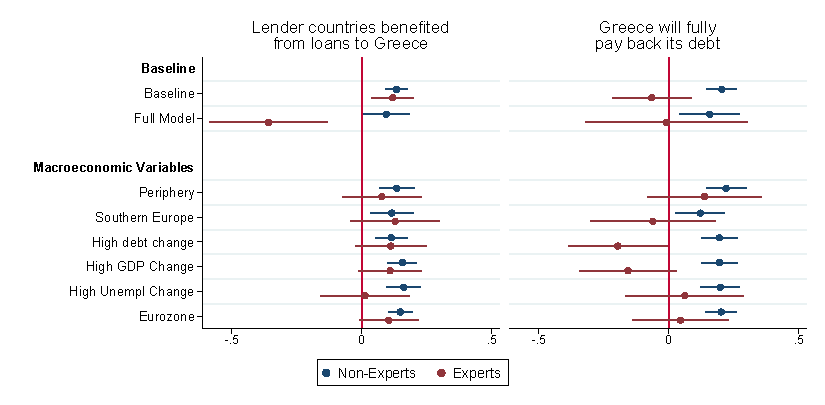
\includegraphics[scale=1.2]{macro_S_1601_S_1701.pdf}
    \end{center}
    \tiny
    \tablenotes{Question 6: Who primarily benefited from the loans to Greece; Question 7: Who primarily benefited from the loans to Greece}
\end{figure}
    \clearpage
\textbf{Ordered and Multinomial Estimation}
In the baseline model we aggregate the response options into two categories, namely whether participants agree or do not agree with a statement.  To examine if differences between participants from non-program and program countries also emerge when we use the full likert scale as the dependent variable we estimate multinomial and ordered logit models. For all questions in which participants were asked to rank their level of agreement we estimate an ordered logit model, for questions in which participants were asked to name the responsible party we estimate a multinomial logit model. Inferences do not change.\\

\\
\textbf{Inattentive Respondents}
When distributing the survey online we included an attention check when asking non-experts about socioeconomic characteristics. All participants failing this attention check were excluded from the survey. We also exclude all participants at the top 10 $\%$ and bottom 10 $\%$ of the survey time distribution. Excluding these participants does not change the inferences of our baseline estimation in the non-expert sample.\\


\\
\textbf{Clustered Robust Standard Errors} 
We cluster standard errors on the country level. Due to the limited number of member states of the European Union we adjust for the small number of clusters using the wild bootstrap method for logit regressions as suggested by \cite{cameron}.\footnote{We use the Stata command developed by \cite{roodman}} Inferences change for some questions when applying this method. The marginal effects fro Question 2.c lack statistical significance, questions 5a and 5c loose some significance and become significant at the 5 and 10 percent level.  \\

\textbf{Multiple Hypothesis Testing}
We also control for multiple hypothesis testing by adjusting our p-values using the Bonferroni Method. We adjust p-values by the number of questions we ask our participants. The Bonferroni correction does not change the significance level of our results. 

%\subsection{Robustness Checks short} 
%Borrower and lender countries vary along other dimensions than the borrower/ lender distinction. Program countries share several characteristics which are likely to influence the estimates. Countries which were affected by the European debt crisis are predominantly Southern European and are located at the periphery of the European Union (measured by distance to Brussels). Further, all these countries experienced a substantial increase in debt levels, high levels of unemployment, low GDP growth and belonged to the Eurozone. Thus we conduct sample splits along these margins to test whether these variables drive our results. \footnote{ We again estimate our model on the subsample of countries which are Southern European, belong to the Eurozone,are located at the periphery of Europe,defined as countries in which the distance of the capital to Brussels is above the median, experienced above median debt and unemployment growth and below median GDP growth during the years 2007 and 2012.} The overall findings of our analysis remain unchanged among the expert and non-expert sample.
%\\
%In addition to controlling for the influence of macroeconomic variables we also conduct several other robustness checks. We estimate the model by ordered and multinomial estimation, we cluster standard errors at the country level, control for multiple hypothesis testing and drop inattentive respondents from our non-expert sample. All these checks do not yield substantially different results than our baseline estimation. A detailed overview of the results of our heterogeneity analysis and robustness checks can be found in the appendix. 
